\documentclass[letter]{scrartcl}

% Use UTF-8 encoding
\usepackage[utf8]{inputenc}
\usepackage{graphicx}

\title{Berlin -- The Pulse of a City}
\author{Tobias Gerken}
\date{\today}


\begin{document}

\maketitle

\section{Introduction}

According to  U.S.~Small Business Association \cite{SBA}, approximately 50\% of new businesses fail within five years of opening. Given the high risk and challenging retail environment, finding the right target demographic and business environment is therefore key. At the same time, cities are becoming increasingly dynamic and diverse which provides ample opportunities for business segmentation. 

Combining data-science approaches with the increasing availability of real time consumer data and open data from city governments can provide valuable insight that can businesses help attract and retain customers.  

\subsection{Business question}
Berlin, the capital of Germany, is home to approximately 3.6 million people and widely recognized to be one of Europe's most dynamic cities. 
Using the city of Berlin as example, we segment its districts by their population demographics and analyze what type of businesses thrive is the respective neighborhoods. The \emph{trending} feature of the Foursquare API, we analyze locations and neighborhoods in Berlin that are trending within a 24-h window letting us experience the \emph{Pulse of the City}.
\\

In detail we ask:
\begin{itemize}
\item Which neighborhoods have the highest density of trending venues?
\item Does the age distribution of district residents have a discernible impact on venues density and type?
\item Can we segment neighborhoods based on the type of business venues they attract and is there a relationship to the demographics Berlin's districts?  
\end{itemize}

\section{Data}

Berlin is a city state divided into 12 districts, each with populations between 200,000 and 400,000 (Figure\ref{fig:Berlin}).  

The Berlin state government provides demographics data for Berlin through its Open Data Portal \cite{Dem}. Geographic shape files of the Berlin districts \cite{Bez} and postcode \cite{PLZ} areas are available through the \emph{Technologie Stiftung Berlin} (Berlin Technology Foundation). 

\begin{figure}[h]
\centering
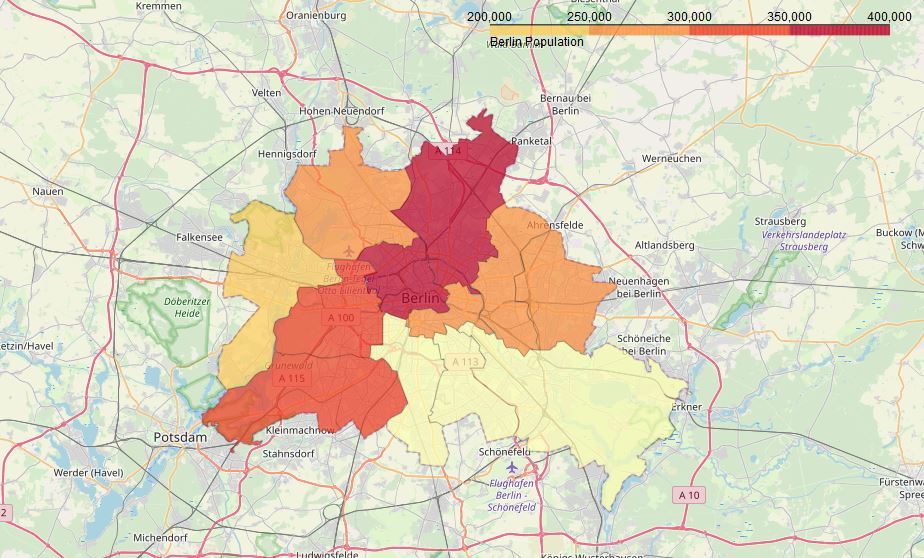
\includegraphics[width=12cm]{../Figures/Berlin_Pop.JPG}
\caption{Berlin is home to 3.6 million people, who live in 12 districts with 200,000 to 400,000 inhabitants each.}\label{fig:Berlin}
\end{figure}

Foursquare's API \cite{FS} allows to query business venue data based on geographical coordinates. Using the \emph{explore} functionality, we receive information about nearby venues, including their postcode and geographic coordinates, which allow them to be linked to Berlin's demographic data. The \emph{trending venues} functionality, allows us to find types of business venues and associated geographic areas that are popular during the course of a day. 

\subsection{Approach}

Demographic data at the city neighborhood-level (\emph{Ortsteil}) were downloaded in CSV-format and aggregated to district level. The demographic data is provided in age groups of 5 years. We suppose that similar age groups have similar consuption patterns and aggregated the data to age groups 0-15, 15-30, 30-50, 60-65, and over 60 years old (Table \ref{tab:demo}), approximately representing children, young adult, middle age, older, and senior consumers. 

\begin{table}[h]
\centering
\caption{There is considerable diversity in age group distribution between Berlin's districts. For example Friedrichshain-Kreuzberg has the larges share of middle age consumers, while Steglitz-Zehlendorf has a much older population.}
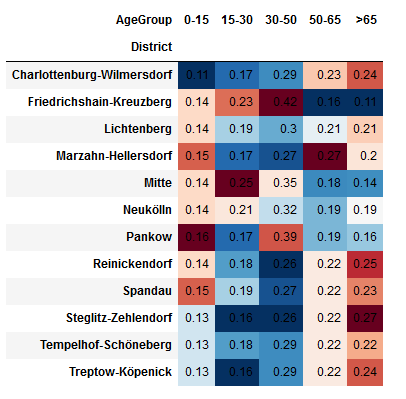
\includegraphics[width=10cm]{../Figures/BerlinTable_color.PNG}
\label{tab:demo}
\end{table}


\subsubsection{Retrieving Venues}

To capture variation in business venues, we execute a gridded sampling approach (Figure \ref{fig:Grid}), where Berlin is covered with an equidistant grid of 1\,km length for which Foursquare search queries are being executed. 

Using the Foursquare API's \emph{explore} functionality, we query recommended venues within a radius of 750\,m around each grid-point. Complete coverage of Berlin is ensured through overlap of the sampling points. Subsequently, duplicate venues are removed. A total of unique 9777 venues were returned. We extracted venue names, venue location, venue address, venue-category and the corresponding city and postcode for each venue. For 1429 venues, for which no postcode was recorded in the data-set, the postcode was retrieved by geographic location using a shapefile of Berlin's postcodes\emph{PLZ}. Finally, we removed any venues for which no postcode could be retrieved, or which had a venue city other then Berlin. This resulted in a final dataset of 9311 venues. 

\begin{figure}[h!]
\centering
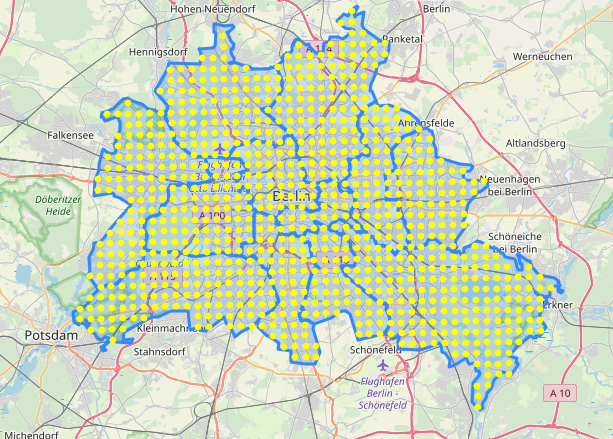
\includegraphics[width=12cm]{../Figures/Grid.JPG}
\caption{The Foursquare API is queried for a large number of locations in Berlin, which are arranged on a regular grid.}\label{fig:Grid}
\end{figure}

Figure \ref{fig:HM} gives an approximation of the venue density in Berlin. However, there is a caveat. The Foursquare API limits the number of returned venues to 50 per search and will only return recommended venues, as such this constitutes a lower bound on the total number of venues in Berlin. 

\clearpage

\begin{figure}[h!]
\centering
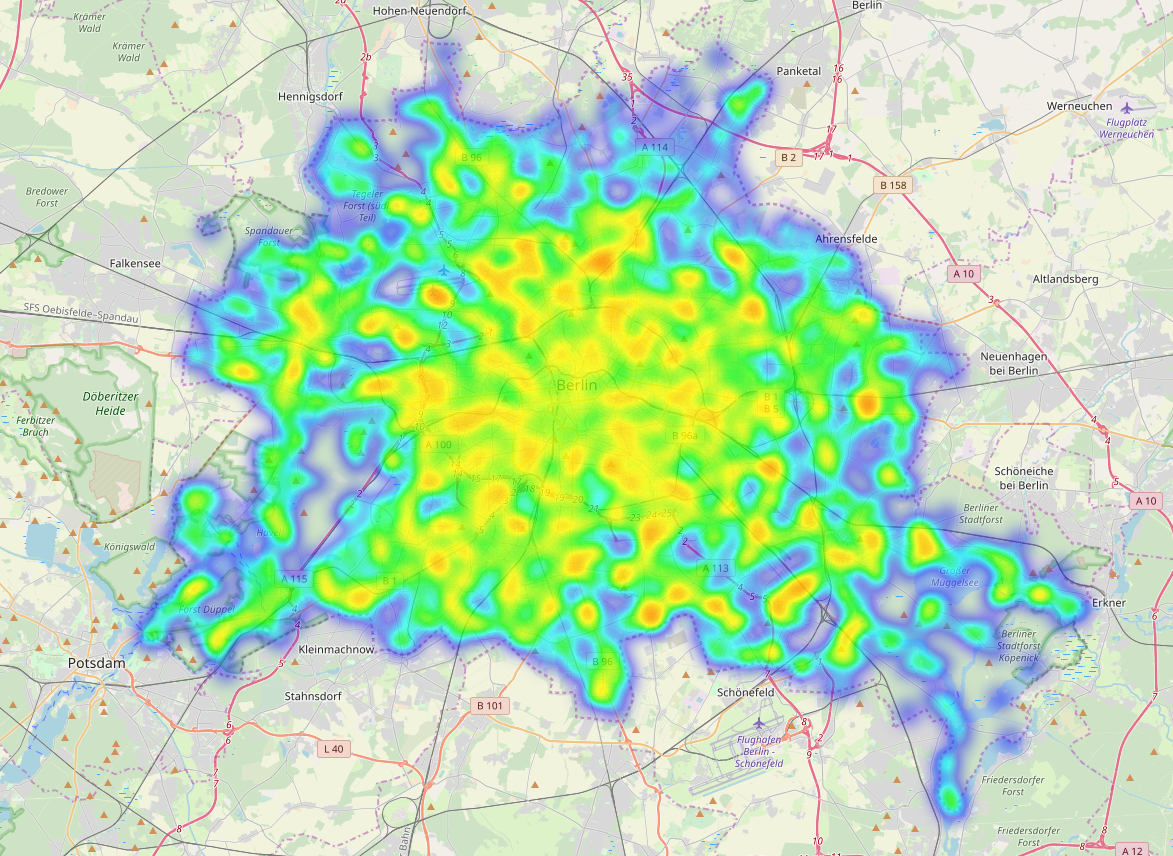
\includegraphics[width=12cm]{../Figures/VenueHM.PNG}
\caption{A total number of 9311 were found almost all over Berlin. The density of venues is notably higher in the center. }\label{fig:HM}
\end{figure}
 
Venues were aggregated by district and by postcode for further analysis. Using the demographics data, we also calculated the venue density as a function of population.  

\begin{figure}[h!]
\centering
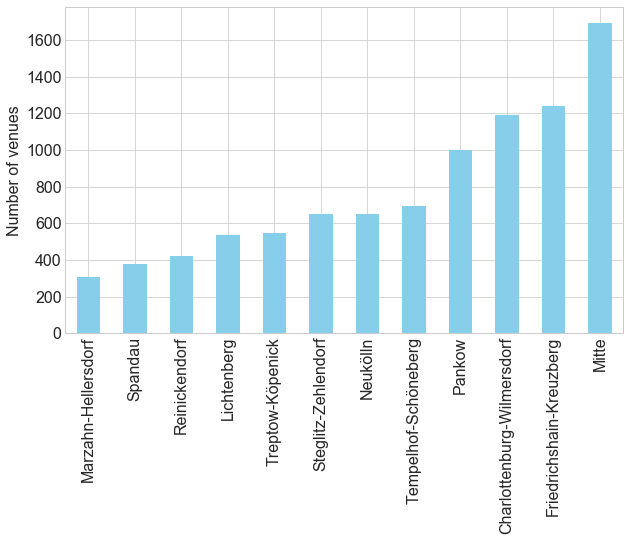
\includegraphics[width=12cm]{../Figures/VenueNumber.PNG}
\caption{The highest number of venues were found in Berlin Mitte ($> 1600$) -- the city center --  and the lowest number of venues were found in Marzahn-Hellersdorf ($\sim 300$) -- a comparatively poor district.}\label{fig:VenNo}
\end{figure}

\subsubsection{K-Means Clustering of Neighborhoods}

To learn more about individual neighborhoods below the district level, we use Berlin's postcode areas as proxy. There are 453 unique venue categories in the data-set. These can be used to learn more about the profile of individual neighborhoods using an unsupervised clustering approach. 

We chose K-Means clustering, one of the most common and computationally cheap clustering algorithms for simplicity. K-Means clustering requires \emph{a-priori} specification of the number of clusters. Given the high number of categories, which leads to sparseness of the data-set, and the fact that we expect neighborhood clusters to not fully separate, we set the number of clusters $K=4$. The K-Means clustering is executed using scikit-learn \cite{sklearn}. We use the venue categories as features for the clustering. Because venue-category is a categorical variable, we create a dummy-variable for each venue category and subsequently normalize the features in each neighborhood to one. 


\subsubsection{Tools}
Data wrangling is performed in Python using Pandas \cite{pd} and Shapely \cite{shapely} (for geospatial calculations).
Visualizations are done using Pyhthon's matplotlib \cite{matplotlib}, seaborn \cite{sns} and Folium \cite{Folium} libraries. 
 
\section{Results}

It is the goal of this report to investigate to detect to \emph{Pulse of the City of Berlin}. To do so we first look into the relationship between demographics and venues found on Foursquare, then investigate further what characterizes neighborhoods in Berlin, and finally follow trending venues over time.

\subsection{Demographics}
Figure~\ref{fig:VenNo} displays the total number of venues for each district. 
Calculating the number of venues per 1000 inhabitants for each district, we can see that the venue density  (Fig.~\ref{fig:VenDens}) closely resembles the total number of venues.  

\begin{figure}[h!]
\centering
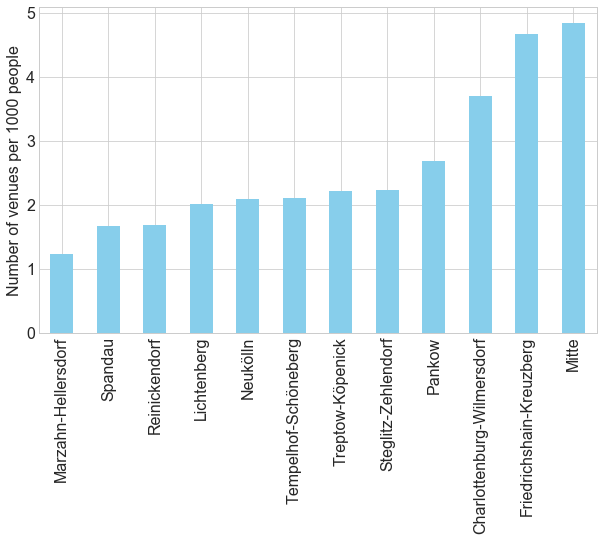
\includegraphics[width=12cm]{../Figures/VenueDensity.PNG}
\caption{The highest number of venues per population were found in Berlin Mitte ($\sim 5$\,venues per 1000 people) -- the city center --  and the lowest number of venues were found in Marzahn-Hellersdorf ($\sim 1$\,venue per 1000 people) -- a comparatively poor district.}\label{fig:VenDens}
\end{figure}

\clearpage 

Interestingly, there is a clear relationship between demography and venue density. We can see that districts that have a higher share of young and middle age adults, have a higher venue density, while  districts with a higher share of people older than 55, have fewer venues per people (Fig.~\ref{fig:PopVsVen}). This may either indicate that younger people actively seek more dynamic living environments or that commercial venues are are more likely to target a younger, wealthier, and more active demographic.

\begin{figure}[h!]
\centering
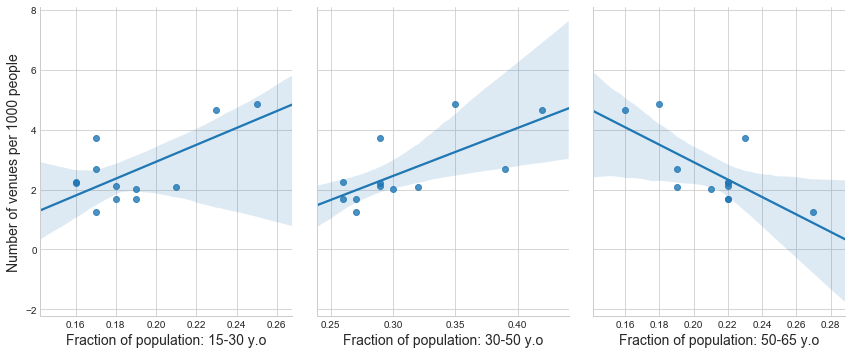
\includegraphics[width=12cm]{../Figures/PopVsVen.PNG}
\caption{There is a clear relationship between demographics and venue density.}\label{fig:PopVsVen}
\end{figure}

\subsection{Clustering of Neighborhoods}

To further investigate the make-up of Berlin, we analyze the venue-data on the neighborhood level. We find that centrally located postcodes have more commercial venues than peripheral postcodes (Fig.~\ref{fig:VenuesPLZ}). 
 
\begin{figure}[h!]
\centering
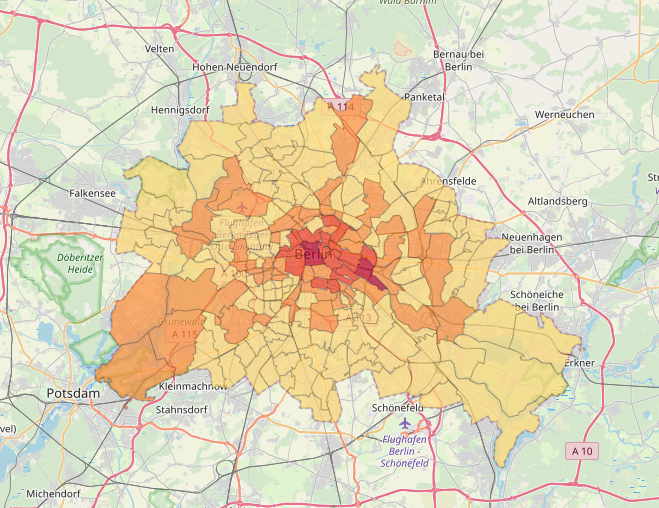
\includegraphics[width=12cm]{../Figures/VenuesMap.PNG}
\caption{The highest number of venues is concentrated near the city center.}\label{fig:VenuesPLZ}
\end{figure}

\clearpage

The clustering results in a 4 clusters. Based on the dominant venues in each cluster, we can investigate the unique features of each cluster.  

\begin{figure}[h!]
\centering
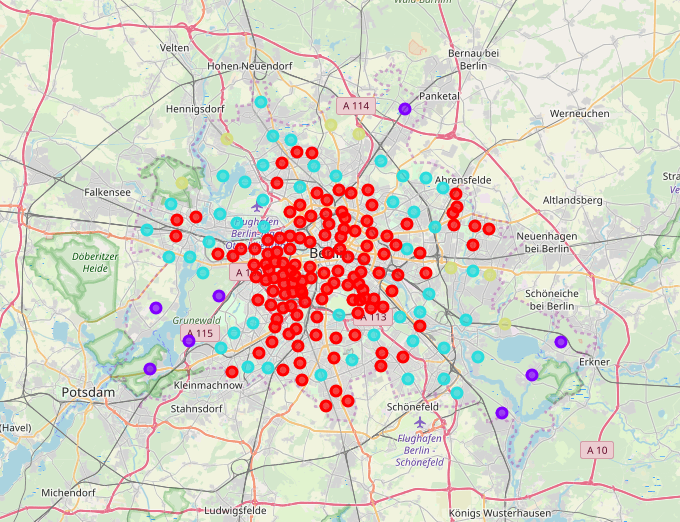
\includegraphics[width=12cm]{../Figures/Clusters.PNG}
\caption{The clustering shows a central cluster which is surrounded by several peripheral clusters.}\label{fig:clusters}
\end{figure}

\begin{description}
	\item[First cluster - The bustling center:] This cluster (indicated in red in Fig.~\ref{fig:clusters}) is located in the center of Berlin. It is dominated by hotels, restaurants, cafes, indicating lots of commercial activity. Hotels indicate tourism for business and pleasure, while cafe's and restaurants contribute to a vibrant atmosphere.  
	\item[Second cluster -People live here \ldots:] This second urban cluster (cyan) is more residential compared to the first urban center. Supermarkes and transit venues are mixed with other commercial venues. These neighborhoods are also located further away from the city center, but still densely built up.
	\item[Third cluster - Respite from the city:] This peripheral cluster (purple) is also  residential with supermarkets and transit venues. At the same time it also features hotels, parks, lakes, marinas, and even a nudist-beach, indicating a recreational quality to be enjoyed by tourists and locals alike. Looking at the map we can also see that lakes, rivers, and forests are nearby confirming our analysis.	
	\item[Fourth cluster -  The city's edge:] This peripheral cluster (green) lacks the attractions of the third cluster. Venues such as parks, fairs, farms indicate lower density. Hotels, forests and lakes indicating recreational activities are largely missing.  
\end{description}


\section{Discussion}


\section{Conclusions}

\begin{thebibliography}{9}
\bibitem{SBA} 
U.S.~Small Business Association: Do economic or industry factors affect business survival? 2012 \\
\texttt{https://www.sba.gov/sites/default/files/Business-Survival.pdf}, 

\bibitem{Dem}
Amt für Statistik Berlin-Brandenburg: Einwohnerinnen und Einwohner in den Ortsteilen Berlins am 30.06.2016, 2016 \\
\texttt{https://daten.berlin.de/datensaetze/einwohnerinnen-}
\texttt{und-einwohner-den-ortsteilen-berlins-am-30062016},   

\bibitem{Bez}
 Technologiestiftung Berlin: Die Bezirksgrenzen der 12 Berliner Bezirke, 2017\\
 \texttt{https://data.technologiestiftung-berlin.de/dataset/bezirksgrenzen}  
  \bibitem{PLZ}
 Technologiestiftung Berlin: PLZ -- Postleitzahlgebiete Berlins, 2015\\
 \texttt{https://data.technologiestiftung-berlin.de/dataset/plz}
 \bibitem{FS}
 Foursquare Labs Inc: Places API, \texttt{https://https://developer.foursquare.com/docs}, Last Access: 4/28/2019
 
\bibitem{sklearn}
scikit-learn, \texttt{https://scikit-learn.org/stable/}, Last Access: 5/11/2019

\bibitem{pd}
Python Data Analysis Library, \texttt{https://pandas.pydata.org/}, Last Access: 5/11/2019

\bibitem{matplotlib}
matplotlib, \texttt{https://matplotlib.org/}, Last Access: 5/11/2019

\bibitem{sns}
seaborn, \texttt{https://seaborn.pydata.org/}, Last Access: 5/11/2019

\bibitem{shapely}
Shapely, \texttt{https://pypi.org/project/Shapely/}, Last Access: 5/11/2019

\bibitem{Folium}
Folium 0.8.3, \texttt{https://python-visualization.github.io/folium/}, Last Access: 5/11/2019


\end{thebibliography}

\end{document}